%%%%%%%%%%%%%%%%%%%%%%%%%%%%%%%%%%%%%%%%%%%%%%%%%%%%%%%%%%%%%%%%%%%%%%%%%%%%%
%	e-Yantra, IIT-Bombay

%	Document Author: Saurav Shandilya
%	Date: 16-August,2012
%	Last Editted by: Saurav
%   Date Last updated: 31-05-2016 

%%%%%%%%%%%%%%%%%%%%%%%%%%%%%%%%%%%%%%%%%%%%%%%%%%%%%%%%%%%%%%%%%%%%%%%%%%%%%

\documentclass[11pt,a4paper]{article}
\newcommand\tab[1][1cm]{\hspace*{#1}}
\usepackage[utf8]{inputenc}

\usepackage{listings}
\usepackage{color}

\usepackage{graphicx}


\title{\textbf{\Huge{Follow Hand}}\vspace{6mm}\\Controlled with leap motion sensor}


\author{Sanket R. Bhimani}
\date{\today}

\begin{document}
	\maketitle
	\newpage
	\tableofcontents
	\newpage
	\section{Tutorial Name:}
	\begin{center}\huge{Robotic Hand Controlled With Leap Motion Sensor}\end{center}
	\tab{This tutorial will help you to making robotic hand which will be controlled with leap motion sensor. Means whatever you perform on leap motion sensor, your hand will perform same thing}
	\vspace{15mm}
	\section{Prerequisites:}
	\vspace{1cm}
	\tab Before going ahead it is better to learn these basic things
    \vspace{1cm}
	\begin{itemize}
	    \item Interfacing servo motors using Galileo Board.
	    \item Knowledge of leap motion library
	    \item Python programming language  and Web socket
	    \item Read Galileo Board tutorial (Recommended)
	\end{itemize}
	\newpage
	\section{Requirement}
	\vspace{1cm}
	\begin{itemize}
	    \item Hardware Requirement:
	    \begin{itemize}
	        \item Galileo Board
	        \item Leap Motion Sensor
	        \item Servo Motors
	        \item Connecting wires
	        \item 3D printed robotic hand (STL files shared in github)
	        \item LAN cable or wifi module(for connecting board with PC)
	        \item Power supply with 4A and 5V (To drive servo motors)
	    \end{itemize}
	    \vspace{1cm}
	    \item Software Requirement:
	    \begin{itemize}
	        \item Python editor
	        \item Leap sdk
	        \item SSH Client
	        \item Linux installed Galileo board
	        \item \textbf{mraa} library
	        \item SSH Client
	        \item Wireshark(optional)
	    \end{itemize}
	\end{itemize}
	\newpage
	\section{Theory and Description}
	\vspace{.3cm}
	\textbf{Introduction:}
	\vspace{.3cm}\\
	\tab{Here, we are trying to control the robotic hand so that it can copy the movements as performed by a subject’s hand over the sensor. The leap motion sensor will detect our hand’s movements and send the acquired data to the Galileo board and board in turn will drive the servo motors. (Refer to Figure 1)}\\
	\vspace{.2cm}\\
	\tab{Finally, according to our hand movements, robotic hand will also move.}\\
	\vspace{1cm}
	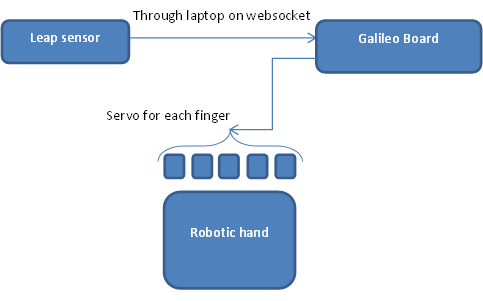
\includegraphics[width=\linewidth]{1.png}
	
	The two things that are needed to implement:\\
	\begin{itemize}
	    \item mapping sensor data with servo angle
	    \item driving servo with Galileo board
	\end{itemize}
	\newpage
	\textbf{Mapping sensor data with servo angle:}
	\vspace{.3cm}\\
	\tab{Here, we want to detect finger movements and according to that we want to find the angle. Thus, we are taking two parameters: Y-axis of palm position and Y-axis of finger’s tip position.}\\
	\vspace{.1cm}\\
	\tab{Afterwards, we are taking “difference of y-axis of palm position and y-axis of finger’s tip position” so we can get the tip position relative to palm position such that the distance from leap motion sensor will not affect the angle.}\\
	\vspace{.1cm}\\
	\tab{This is done in order to make sure that we can easily perform pose at any place in range of leap motion sensor.}\\
	\vspace{.1cm}\\
	\tab{Then this value is mapped with the servo angle. The range of servo angle can be obtained using trial and error method. }\\
	\vspace{.1cm}\\
	\tab{This way we can find all finger angles and this angle data is sent to Galileo board and board will drive servo according to angle value.}\\
	\newpage
	\textbf{Driving servo with Galileo board:}
	\vspace{.3cm}\\
	\tab{For that initially I was trying to achieve that with SYSFS. But here time\_period of 20 millisecond is not acceptable so I couldn’t use that way. And all other library is also based on this system. But only MRAA is different it directly contact with microcontroller and do such things. Because from arduino IDE I could run servo, It means board is capable but software is bottle necking somehow. So, Finally using MRAA library it become easy.}\\
	\vspace{.2cm}\\
	\tab{For driving servo with Galileo board, we need to generate PWM signal. For that purpose, MRAA library has been put to use.}\\
	\vspace{.2cm}\\
	\tab{Here PWM signal’s time period should be 20 millisecond and duty cycle should be 1 to 2 milliseconds.}\\
	\vspace{1cm}
	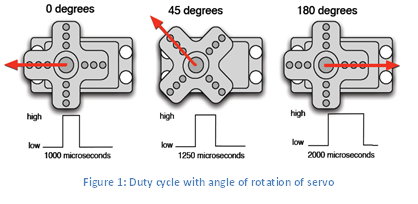
\includegraphics[width=\linewidth]{2.png}
	\vspace{.3cm}\\
	\textbf{Note: }In the project however, I have used 4640 microsecond! As on 20 millisecond it was not working properly. So, I’ve found this value from trial and error method and it is working properly now. So if you are trying to make such thing then first try 20 milliseconds as time period.
	\newpage
	\vspace{.3cm}
	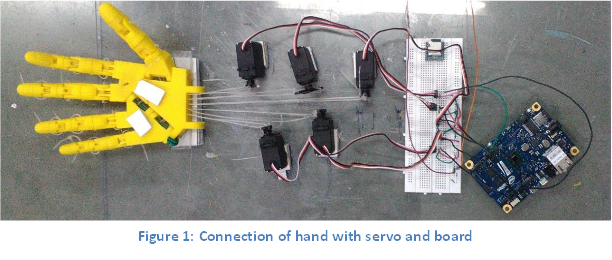
\includegraphics[width=\linewidth]{3.png}
	\vspace{.3cm}
	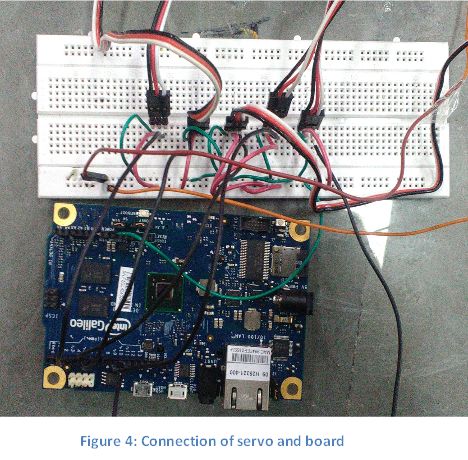
\includegraphics[width=\linewidth]{4.png}

	
	\newpage
	\textbf{Connection:}
	\vspace{.3cm}\\
	\tab{Here pins marked with “~” are PWM pins. Connect servo’s signal pin with this pins. And give 5V to each servo. And make sure that voltage doesn’t drop. For that, give at least 4A current among all the servos.}\\
	\vspace{1cm}
	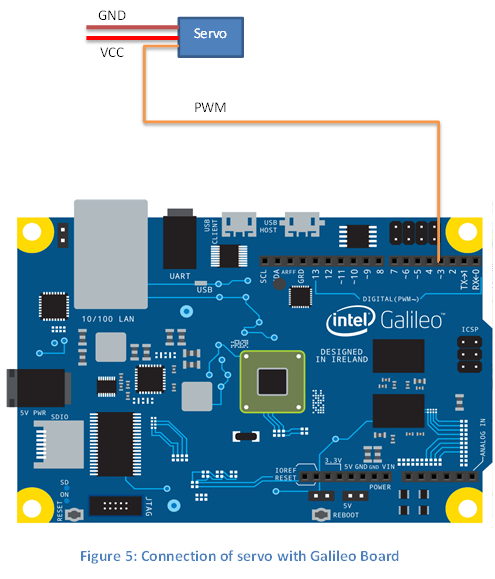
\includegraphics[width=\linewidth]{5.png}
	\vspace{.3cm}
    \newpage
	\section{References}
	\begin{itemize}
	    \item http://www.instructables.com/id/Robotic-Hand-controlled-by-Gesture-with-Arduino-Le/step2/Make-the-Hand/
	    \item https://github.com/LikeFace/FollowHand
	    \item http://inmoov.fr/hand-and-forarm/
	    \item http://inmoov.fr/finger-starter/
	    \item https://github.com/intel-iot-devkit/mraa/
	    \item http://sweb.cityu.edu.hk/sm2240/4/sevro\_2.png
	\end{itemize}
\end{document}



